\chapter{Evaluation of results}
\label{evaluation}
In~this chapter, individual recognition phases are evaluated. Some evaluation of~YOLOv7 training strategies was already done in~section~\ref{design-keyboard-implementation}. There were discussed differences between~16~vs.~32~batch size and finetuning vs. new training. Furthermore,~three~versions of~640x640~YOLOv7 models were introduced. The following sections~\ref{evaluation-keyboard} and~\ref{evaluation-chars} present the comparison of the YOLOv7 variations (yolov7-tiny, yolov7, yolov7-x) and discuss the choices made. The last section~\ref{evaluation-postprocessing} shows results of~the post-processing algorithm on~its validation dataset. The metrics used for the evaluation are precision, recall and for~the YOLOv7 models also mAP. The mAP was computed for~0.5 and~0.95 intersection-over-union values. A~full account of~the results is available on~the attached medium~\ref{Appendix-A}, here only selected metrics and results are used for~demonstration.

\section{Keyboard detector}
\label{evaluation-keyboard}
As~described in~section~\ref{design-keyboard-implementation}, yolov7-tiny is smaller, faster and uses fewer resources than the original YOLOv7 variation from the paper~\cite{yolov7} at~the cost of~accuracy. On~the contrary, yolov7-x is supposed to~be more accurate at~the cost of~reduced processing speed, higher resource consumption and bigger size. Figure~\ref{eval-keyboard-resources} illustrates the comparison in~resource consumption on~averaged memory allocation in~percents on~a \hbox{2-core} GPU provided by~Kaggle platform. The relative difference between the models is very similar in~GPU utilization and other physical metrics as well. Another factor is the actual size of~the models. The tiny model has only about~12~KB, while the original one takes about~73~KB and the yolov7-x even~140~KB. So~far, the tiny version is the winner. The comparison of~mAP@.95 metric development during the training, which gives an account of~the accuracy properties of~the models, is shown in~figure~\ref{eval-keyboard-training}. Recall, precision and loss functions are available on~the attached medium~\ref{Appendix-A}, but as~mAP is dependent upon recall and precision, it is a sufficient representation of~the detector's overall capabilities. As~can be seen, the training progressed very similarly and all 3~models came to the same results. This proves that for the keyboard detection task, the bigger models do not bring any additional value. Hence, the yolov7-tiny version is used as it is as accurate as the other versions while being significantly faster and requiring fewer computational resources. The full account of~the training results on~the testing dataset is in~table~\ref{eval-table-keyboard}. Apart from mAP@.95 the results are identical. There can be seen a slight improvement in~mAP@.95 among the bigger models, but that can be viewed as~insignificant. The~near~2~\% difference between yolov7-tiny and yolov7-x is negligible especially if taking into consideration the cost of~size, speed and resources.

\begin{figure}[hbt]
    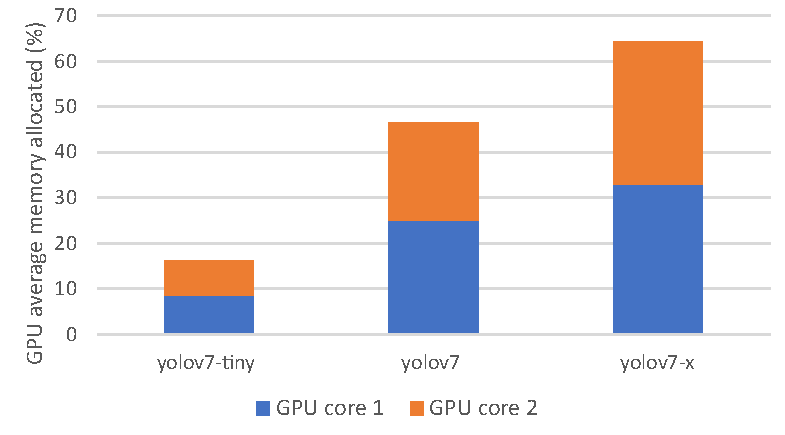
\includegraphics[width=1\textwidth]{img/evaluation/eval-keyboard-resources.pdf}
    \caption{The tiny version of~the YOLOv7 proves to be substantially more efficient in~terms of~resource consumption. Comparisons of~other physical metrics look fairly similar.}
    \label{eval-keyboard-resources}
\end{figure}

\begin{figure}[!hbt]
    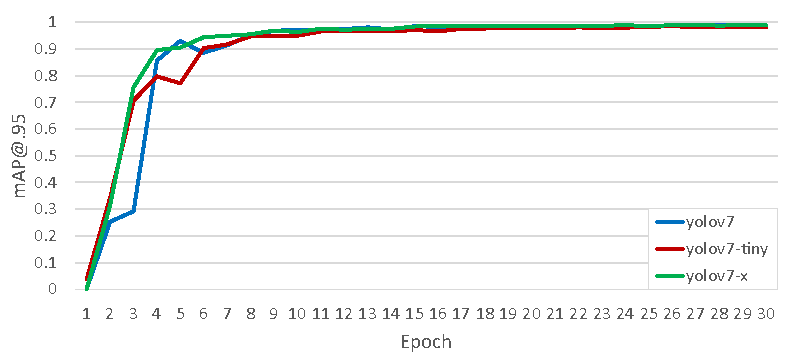
\includegraphics[width=1\textwidth]{img/evaluation/eval-keyboard-training.pdf}
    \caption{The development of~mAP@.95 on~validation data during training indicates a minimal difference in~the expressive power of~the models.}
    \label{eval-keyboard-training}
\end{figure}

\vspace{12pt}
\begin{table}[!hbt]
\begin{tabular}{
|p{0.2\textwidth}|>{\centering\arraybackslash}p{0.164\textwidth}|>{\centering\arraybackslash}p{0.164\textwidth}|>
{\centering\arraybackslash}p{0.164\textwidth}|>
{\centering\arraybackslash}p{0.164\textwidth}|}
 \hline
 \centering Model & Precision & Recall & mAP@.5 & mAP@.95\\
 \hline
 yolov7-tiny & 1 & 1 & 0.996 & 0.971 \\
 yolov7 & 1 & 1 & 0.997 & 0.98 \\
 yolov7-x & 1 & 1 & 0.997 & 0.989 \\
 \hline
\end{tabular}
\caption{The results of~individual models on~the testing keyboard dataset show that all of~them are almost equally accurate.}
\label{eval-table-keyboard}
\end{table}

\section{Character detector}
\label{evaluation-chars}
Due to using the same model as for the keyboard detection, the character detector was evaluated in~the same manner. Concerning resource consumption, the difference between the models got reduced as~can be seen in~figure~\ref{eval-char-resources}. The tiny model is still the clear winner, but not as~notably as~in~keyboard detection shown in~figure~\ref{eval-keyboard-resources}. This is caused by~the increased number of~classes and thus a greater number of~detections made.

\begin{figure}[hbt]
    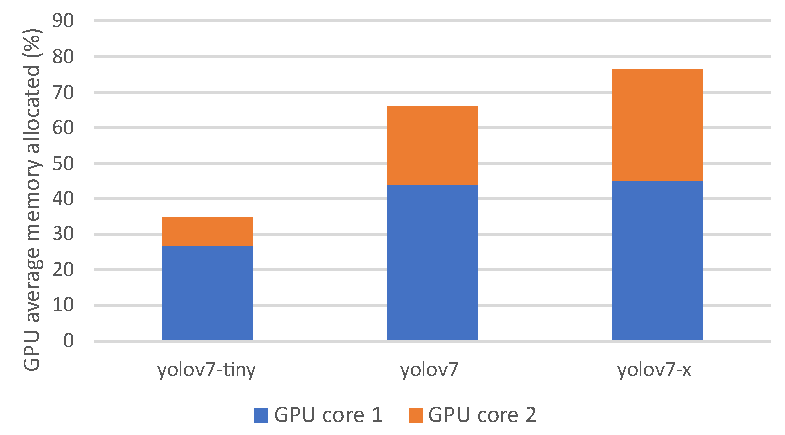
\includegraphics[width=1\textwidth]{img/evaluation/eval-char-resources.pdf}
    \caption{The resource consumption is a bit more leveled than in~keyboard detection, but the fact that the bigger the model the higher the consumption still holds. Again, other metrics such as~GPU utilization show similar differences.}
    \label{eval-char-resources}
\end{figure}

When it comes to~the expressive power of~the models, the tiny model falls behind as~demonstrated by~figure~\ref{eval-char-training}. The bigger models are again almost identical, with the difference that yolov7-x was trained slightly smoother. The higher number of~classes and presumably some similar-looking characters are problematic for the tiny model though. Nevertheless, it is still quite sure with itself as~figure~\ref{eval-char-training-precision} shows. While it still cannot reach the same precision as~the bigger models and it climbs slower, it eventually comes close. The problem lies in~recall where the chart looks similar to~figure~\ref{eval-char-training}. It simply cannot detect as~many characters and the ones detected have lower confidence scores. The complete results are laid out in~table~\ref{eval-table-chars}. The yolov7-x version again does not bring any improvement so due to its size it is considered no more. Thus, the original YOLOv7 model is selected for~the character recognition task. However, the next section~\ref{evaluation-postprocessing} explains why the tiny model might still be of~use. The presented data are overall results. Character-specific metrics are available on~the attached medium~\ref{Appendix-A}. To demonstrate the accuracy variability of~individual characters, figure~\ref{eval-char-f1} shows their F1 curves. The lowest curves belong to special characters such as~dot, comma or underscore while the top ones are for special key icons and capital alphabet characters. In~conclusion, it is visible that the accuracy varies which was expected not only because of~special characters but also non-discriminative upper and lower case letters.

\begin{figure}[hbt]
    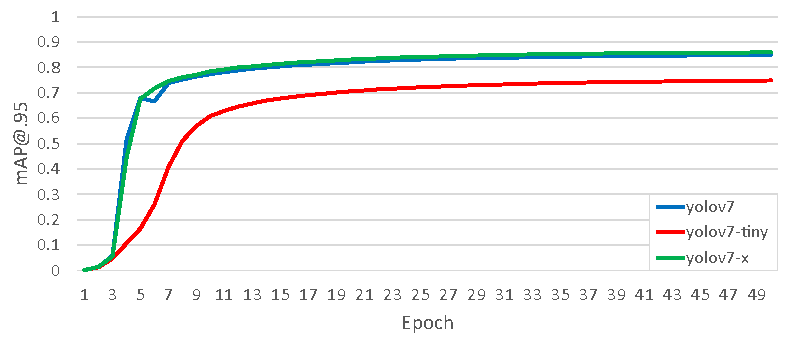
\includegraphics[width=1\textwidth]{img/evaluation/eval-char-training.pdf}
    \caption{The development of~mAP@.95 on~validation data during training indicates that bigger yolov7-x is not stronger that the normal version. However, in~comparison with the keyboard detector, the tiny version is not as~accurate~as the bigger models.}
    \label{eval-char-training}
\end{figure}

\vspace{12pt}
\begin{figure}[!hbt]
    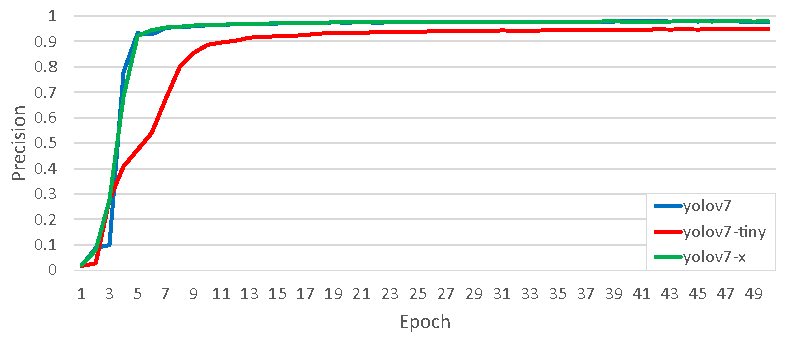
\includegraphics[width=1\textwidth]{img/evaluation/eval-char-training-precision.pdf}
    \caption{The development of~precision on~validation data during training shows that the bigger models have the same precision. The tiny version falls behind a bit but it is still competitive.}
    \label{eval-char-training-precision}
\end{figure}

\begin{table}[!hbt]
\begin{tabular}{
|p{0.2\textwidth}|>{\centering\arraybackslash}p{0.164\textwidth}|>{\centering\arraybackslash}p{0.164\textwidth}|>
{\centering\arraybackslash}p{0.164\textwidth}|>
{\centering\arraybackslash}p{0.164\textwidth}|}
 \hline
 \centering Model & Precision & Recall & mAP@.5 & mAP@.95\\
 \hline
 yolov7-tiny & 0.948 & 0.852 & 0.912 & 0.748 \\
 yolov7 & 0.979 & 0.951 & 0.977 & 0.848 \\
 yolov7-x & 0.98 & 0.95 & 0.978 & 0.858 \\
 \hline
\end{tabular}
\caption{The results of~individual models on~the testing character dataset show that while the tiny model is less accurate, especially in~terms of~recall and mAP@.95, the difference between the normal and bigger versions is minuscule.}
\label{eval-table-chars}
\end{table}

\begin{figure}[hbt]
    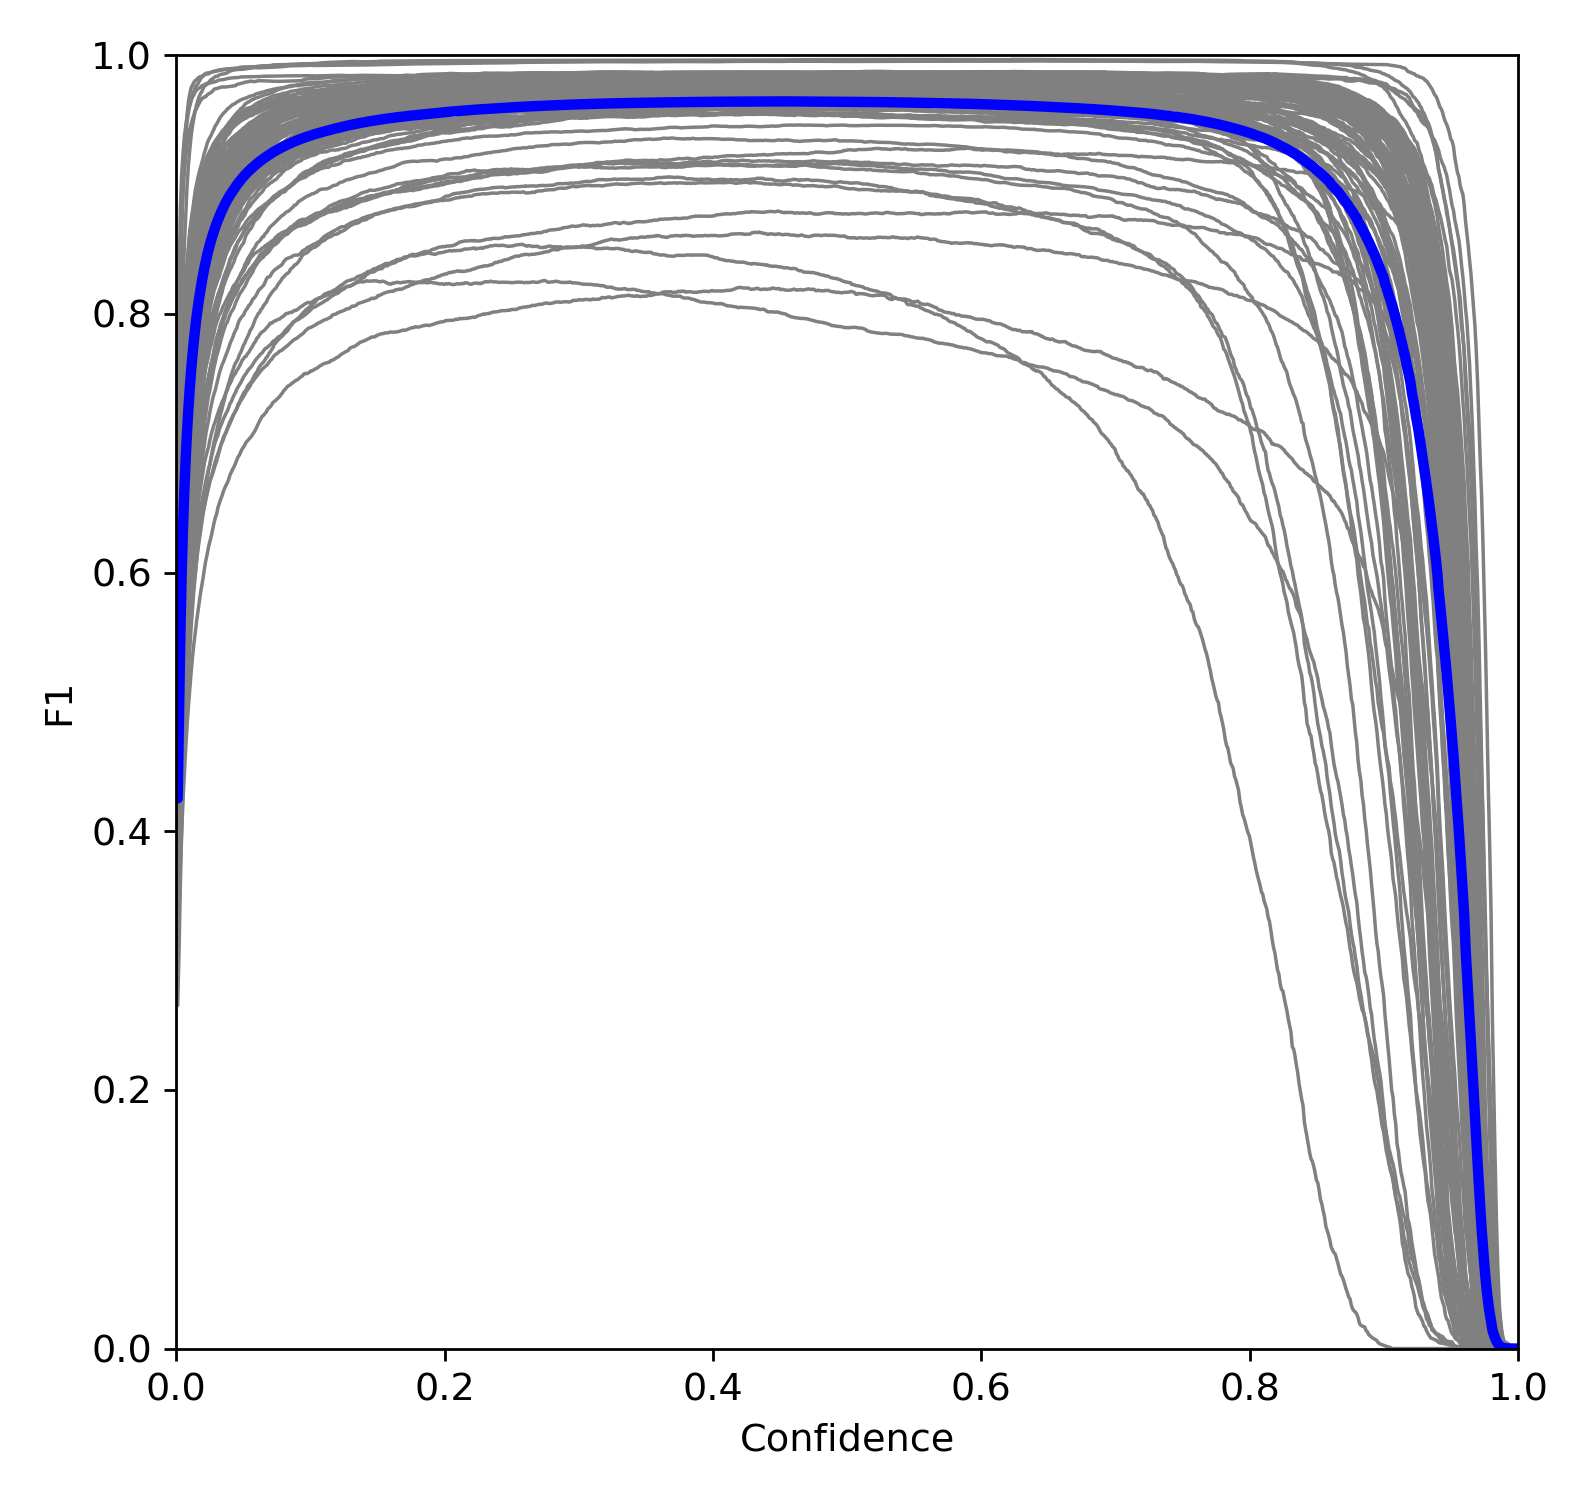
\includegraphics[width=0.95\textwidth]{img/evaluation/eval-char-f1.png}
    \caption{The majority of F1 curves for individual characters (gray) is better than the overall F1 curve (blue) from the original YOLOv7 model on~character testing dataset. This is due to some less accurate special characters.}
    \label{eval-char-f1}
\end{figure}

\section{Post-processing algorithm}
\label{evaluation-postprocessing}
The character detector's results show that there is room for~improvement. The post-processing algorithm not only improves overall recognition results but also removes the accuracy gap between the tiny and normal models. On~the post-processing validation dataset, the character recognition with applied post-processing achieves similar though slightly worse results shown in~table~\ref{eval-postprocessing-table} than the single-character detection on~the \hbox{character} dataset. Notwithstanding, the results are still impressive considering this is a real-world and not a~generated dataset. Moreover, these are averaged numbers impaired with special character detection on which not much post-processing is done.

As~the table shows, the results for special characters are nowhere near as good as for the other keys. Partially, it is due to dots~vs.~noise/commas/colons/semicolons or underscores~vs.~dashes etc. It may to a degree be also due to some low-quality validation images. As~not many full-HD samples could be obtained, the dataset consists of~keyboards of~diverse quality. It can be presumed that on~full-HD images from~AIVA cameras, the results might be slightly better. It is worth reminding, that special character recognition was not the main objective so~for a bonus the results can still be considered satisfactory.

The special keys results are significantly better. Though they are not yet perfect, \hbox{taking} into account that these keys do not have to have just icons but also words on~them, the results are favorable. The letters in~words are usually much smaller than on~regular keys, hence harder to recognize. Furthermore, because of~the close proximity to~other characters in~the word, the detector can be easily baffled, especially in~lower-quality images. Consequently, joining letters to~words and recognizing the words in~spite of~missing (undetected or incorrectly detected) letters with such precision and recall is considered a success.

Despite special characters not doing so well, the results for target alphanumeric characters exceed expectations and show how powerful the post-processing really is. The reason for this is quite simple. Let's consider a qwerty layout. All the detector needs to recognize is one character in~each row and at~least a minimum-requirement number of~characters in~a row for the layout to~be recognized as~qwerty. This gives the algorithm a starting point and both \emph{x} and \emph{y} distances between characters. The rest can be computed or corrected with almost~100~\%~accuracy. As~a~consequence, the detector's responsibility is to provide just a bare minimum. This is also the reason why the tiny model actually performs slightly better. It does not produce as~many false positives to~confuse the algorithm as~the normal version does and the undetected characters can be easily computed.

\begin{table}[hbt]
\begin{tabular}{
|p{0.2\textwidth}|>{\centering\arraybackslash}p{0.164\textwidth}|>{\centering\arraybackslash}p{0.164\textwidth}|>
{\centering\arraybackslash}p{0.164\textwidth}|>
{\centering\arraybackslash}p{0.164\textwidth}|}
\hline
& \multicolumn{2}{c|}{yolov7} & \multicolumn{2}{c|}{yolov7-tiny}\\
 \hline
 & Precision & Recall & Precision & Recall\\
 \hline
 All keys & 0.942 & 0.949 & 0.964 & 0.942\\
 Alphabet & 1 & 1 & 1 & 1\\
 Numbers & 0.998 & 0.987 & 1 & 0.993\\
 \textbf{Alphanumeric} & \textbf{0.999} & \textbf{0.997} & \textbf{1} & \textbf{0.998}\\
 Special keys & 0.965 & 0.910 & 0.987 & 0.914\\
 Special characters & 0.684 & 0.767 & 0.762 & 0.705\\
 \hline
\end{tabular}
\caption{Among the results of~the post-processing algorithm on~the validation dataset stand out alphanumeric characters.}
\label{eval-postprocessing-table}
\end{table}